\documentclass[12pt,a4paper,oneside]{book}
\usepackage{amsmath}
\usepackage{amssymb}
\usepackage{amsthm}
\usepackage{graphicx}
\usepackage{latexsym}
%\usepackage{pslatex}
\usepackage{color}
\usepackage{fancyhdr}
\usepackage{cite}
\usepackage{indentfirst}
\usepackage{tocloft}
\usepackage{multirow}
\usepackage{fontspec}

% Times New Roman
\setromanfont[
BoldFont=Times New Roman Bold.ttf,
ItalicFont=Times New Roman Italic.ttf,
BoldItalicFont=Times New Roman Bold Italic.ttf,
]{Times New Roman.ttf}
%\setmainfont{Times New Roman}

% Centering Chapter
\usepackage{sectsty}   
\chapterfont{\centering}

\pagestyle{myheadings}
\setlength{\parindent}{0.8in}

\usepackage[top=1.5in,bottom=1in,left=1.5in,right=1in]{geometry}



% Theorem style-------------------------------------------------------------------
\theoremstyle{plain}
\newtheorem{thm}{Theorem}[chapter]
\newtheorem{lem}[thm]{Lemma}
\newtheorem{cor}[thm]{Corollary}
\newtheorem{prop}[thm]{Proposition}
\newtheorem{rem}[thm]{Remark}
\newtheorem{ex}[thm]{Example}
\newtheorem{de}[thm]{Definition}
\renewcommand{\proof}{\textbf{Proof.}}

\numberwithin{equation}{chapter} \DeclareMathOperator{\Var}{Var}
\DeclareMathOperator{\Ima}{Im}

\usepackage{float}
%\usepackage[skip=2pt,font=footnotesize]{caption}

% Graph-------------------------------------------------------------------
\usepackage{graphics,graphicx}
\usepackage{calc}
\usepackage{tikz}
\usetikzlibrary{decorations.markings}
\tikzstyle{vertex}=[circle, draw, inner sep=2pt, minimum size=4pt]
\newcommand{\vertex}{\node[vertex]}
\newcounter{Angle}

% Line space-------------------------------------------------------------------
\renewcommand{\baselinestretch}{1.5}

\newcommand*{\QEDA}{\hfill\ensuremath{\large{\lozenge}}}
\newcommand*{\QEDAa}{\hfill\ensuremath{\square}}

\renewcommand{\bibname}{\centerline{\Large REFERENCES}}

%Centering table of contents and list of table
\usepackage{tocloft}
\renewcommand{\contentsname}{\hfill\bfseries\Large TABLE OF CONTENTS \hfill}   
\renewcommand{\cftaftertoctitle}{\hfill}

\renewcommand{\listtablename}{\hfill\bfseries\Large LIST OF TABLES} 
\renewcommand{\cftafterlottitle}{\hfill}

\renewcommand{\listfigurename}{\hfill\bfseries\Large LIST OF FIGURES} 
\renewcommand{\cftafterloftitle}{\hfill}







\begin{document}
\thispagestyle{empty}

\begin{figure}[h!]
\vskip1in
\begin{center}

\includegraphics[width = 3.5 cm]{ruhuna.png}
\end{center}
\end{figure}

\begin{center}
\large{\textbf{WATER LEVEL INDICATOR}}
\end{center}

\vskip2.5mm

\begin{center}
\textbf{BY}
\end{center}

\vskip0.6cm

\begin{center}
\textbf{E.S.K.CHANDRASEKARA}\\
\textbf{W.K.T.KANCHANA}\\
\textbf{M.C.MANAGE}\\
\textbf{H.P.P.ERANDI}\\
\textbf{K.D.THENUWARA}
\end{center}

\vskip1.0cm
 
\begin{center}
\textbf{AN ASSIGNMENT SUBMITTED IN ELECTRONIC COURSE}
\end{center}

\begin{center}
\textbf{PHY 2112}
\end{center}
\vskip1cm
\begin{center}
\textbf{DEPARTMENT OF PHYSICS}
\end{center}
\begin{center}
\textbf{FACULTY OF SCIENCE}
\end{center}
\begin{center}
\textbf{UNIVERSITY OF RUHUNA}
\end{center}


\newpage
\pagenumbering{roman}
\begin{table}[h]
	\begin{tabular}{ll}
		Project Title								   & WATER LEVEL INDICATOR  \\
										 				
		By							   					  & Chandrasekara ESK (SC/2018/10559) \\
															& Kanchana WKT (SC/2018/10656)  \\
															& Manage MC (SC/2018/10660) \\ 
															& Erandi HPP (SC/2018/10568) \\
															& Thenuwara KD  (SC/2018/10657) \\
		Field of Study			  					 & Mathematics, Computer science, Physics, Electronic,

\\
		Project Advisor								& DR. Sameera Lakshan \\
															
		Academic Years							  & 2020 \\
	\end{tabular}
\end{table}
\begin{center}
  \large{\textbf{ABSTRACT}}\\
\end{center}
\addcontentsline{toc}{chapter}{ABSTRACT}

Water tank overflow is a common problem which leads to the wastage of water. Though there are many solutions to it like ball valves which automatically stop the water flow once the tank gets full .But being electronics enthusiastic wouldn't you like an electronic solution for it. So here is simple process that will guide you to make a circuit which will detect the water level and will light LED bulbs upon getting the water tank full or a preset  level.
\
This simple transistor based water level indicator circuit is very useful to indicate the water levels in a tank. Whenever tank gets filled, we get alerts on particular levels. In here we have created 4 levels in a tank.(low,medium,high and full), We have to added 4 LEDs to indicate four levels.LED bulbs light up at each levels. 



\newpage
\begin{center}
	\large{\textbf{ACKNOWLEDGEMENTS}} \\
\end{center}
\addcontentsline{toc}{chapter}{ACKNOWLEDGEMENTS}


In performing our assignment, we had to take the help and guideline of some respected persons, who deserve our greatest gratitude.The completion of this assignment gives us much pleasure. We would like to show our gratitude \textbf{Dr.Sameera Lakshan, Course Instructor, University of Ruhuna}  for giving us a good guideline for assignment throughout numerous consultations. We would also like to expand our deepest gratitude to all those who have directly and indirectly guided us in writing this assignment.
 

%\vspace{0.4cm}


%\renewcommand{\contentsname}{TABLE OF CONTENTS}

\newpage

%\pagenumbering{roman}
%\addcontentsline{toc}{chapter}{LIST OF TABLES}
\tableofcontents
%


\newpage
\addcontentsline{toc}{chapter}{LIST OF FIGURES}
\listoffigures

\newpage
\addcontentsline{toc}{chapter}{LIST OF TABLES}
\listoftables


\newpage
\pagenumbering{arabic}
\chapter{INTRODUCTION}
Generally, when the tank is full, water contained in the overhead tank is lost caused by excessive flow. The overflow of water tanks is a common issue that results in water wastage we see in our day today life. And though there are many alternatives to it as ball valves that stop the flow of water automatically until the tank gets full. But being passionate about technology, we would like to introduce you to an electronic solution for it.

Nowadays all householders use pumps to store the water in overhead tanks. No one else can identify the water level when the water is stored in the tank, and thus no one will tell whenever the water tank will fill. Therefore, there is an overflow of water in the tank, so there is a loss of water and electricity.

As a solution, a simple mechanism for detecting and showing the level of water in the overhead tank and even in the other containers is the water level alarm circuit. It helps and displays the level of water in the overhead tanks to solve this sort of problem by using the water level warning circuit. The low cost of the water level warning circuit is because it is used exclusively for water tanks, boilers for swimming pools, etc.  And this kind of applications are used in the factories, chemical plants, and electrical substations and also in other liquid storage systems as well.



\chapter{REVIEW OF LITERATURE}

\section{Water Level Indicator}\label{Sec2.1}

The indicator of the water level is defined as a device that obtains information on the water level in reservoirs or tanks used during homes. We can solve the overflow of water from the tankers by using the water level indicator.

\begin{figure}[hbt!]
    \centering
    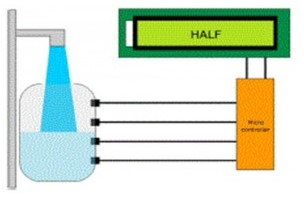
\includegraphics{a.jpg}
    \caption{Water Level Indicator}
    \label{fig:a}
\end{figure}

\section{Purpose of Water Level Indicator}

Nowadays, The saving of water is a critical problem that requires instantaneous and potential attention. Every day a number of gadgets are coming onto the market to help human beings minimize the loss of water. One such instrument is the water degree indicator. It has a very easy to recognize mechanism. The water level indicator monitors and displays the water level in the overhead water tank or other water tanks. 

When the water is contained within the tank, nobody else can confirm the degree of water, although it can be difficult to determine when the water tank is being filled. Most people know that the tank is full as the water begins to drain out of the tank.
Therefore approaches there may be a waste of water and electricity.

\section{Components Required}
This simple transistor based water level indicator circuit is very useful for indicating the water level in the tank. To create this circuit the below-mentioned apparatus was used to make it a success. 

\subsection{Transistors}

    
There are three terminals in the transistor, namely emitter $(E)$, base $(B)$, and collector $(C)$. We've got two types of transistors, $npn$ and $pnp$.
\begin{figure}[hbt!]
    \centering
    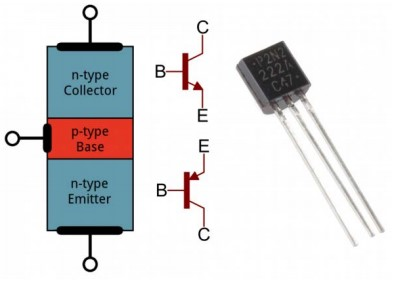
\includegraphics{b.jpg}
    \caption{Two types of transistors $npn$ and $pnp$}
    \label{fig:b}
\end{figure}

\newpage
The only difference between the $npn$ and the $pnp$ is the path of the arrow to the emitter. The arrow on the $npn$ points out and it points to the $pnp$ as shown in figure \ref{fig:b}. 

And also transistors are something of an extension of yet another semiconductor component, diodes. In such a way, the transistors are just two diodes with their cathodes (or anodes) connected.

\begin{figure}[hbt!]
    \centering
    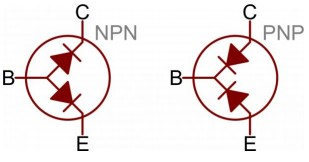
\includegraphics{c.jpg}
    \caption{A Transistor as Two Diodes}
    \label{fig:c}
\end{figure}

To construct this circuit we had to use BC547 transistors and BC547 is an $npn$ transistor such that the collector and emitter are left open (Reverse bias) while the base pin is placed to the ground and closed (Forward bias) when the base pin is signaled. The maximum total current which would flow through the collector pin is $500mA$, so we cannot connect loads that produce more than $500mA$ using that same transistor. Which means we have to supply current to base pin, this current $(I_{\beta})$ should be limited to $5mA$.

\begin{figure}[hbt!]
    \centering
    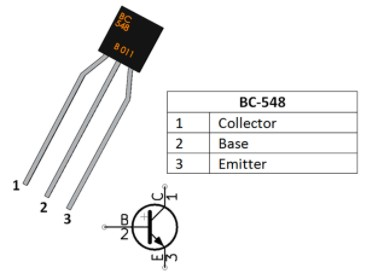
\includegraphics[width=0.5\textwidth]{d.jpg}
    \caption{BC547 transistors}
    \label{fig:d}
\end{figure}

\newpage

\subsection{Resistors}
Resistors are materials used to withstand the flow of electrical current and have a given resistance value. Many types of resistors have different uses and constructions. There are two general types of resistors that you can use as an installer. They are fixed and variable resistors. The most popular forms have a fixed resistance value, so they are also referred to as fixed resistors. They are shown in circuit schematic diagrams using one of the symbols shown in Figure \ref{fig:e}.

\begin{figure}[hbt!]
    \centering
    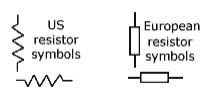
\includegraphics[width=0.7\textwidth]{e.jpg}
    \caption{Resistor symbols}
    \label{fig:e}
\end{figure}

Different kinds of fixed resistors are used in circuits, are the most numerous of all electronic devices, with their most commonly used approach is to minimize voltages and currents across the circuit. Resistors are often used in combination with other elements, such as inductors and capacitors, to process signals in several ways. Since resistors are 'passive elements' that cannot intensify or increase voltages, currents, or signals, they can only minimize them. However, they are the most important part of any electronic circuit.

Resistors are selected for the amount of resistance they posses. This value is measured in Ohm’s $(\Omega)$. Then we consider about resistors value calculation almost all of the fixed value resistors are labeled with a set of color-coded bands wrapped around the resistor.

In Figure \ref{fig:g}, five color bands are shown around the resistor. Note also that these color bands are oriented towards one end of the resistor. They are read from left to right starting with the far left
band. 

\newpage

\begin{figure}[hbt!]
    \centering
    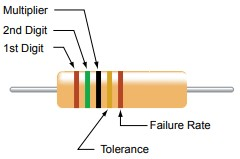
\includegraphics[width=0.5\textwidth]{g.jpg}
    \caption{Resistor value calculation}
    \label{fig:g}
\end{figure}

\begin{itemize}
    \item \textbf{The first three (3) band} have to do with the value of the resistor in resistance (Ohms). 
    \item \textbf{The fourth (4) band}  (if present) identifies the accuracy or Tolerance of the resistor. 
    \item \textbf{The fifth (5) and final band} (if present) indicates the failure rate of the resistor.
\end{itemize}

\begin{figure}[hbt!]
    \centering
    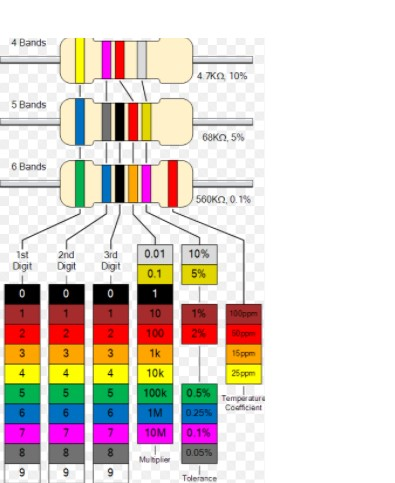
\includegraphics[width=0.5\textwidth]{j.jpg}
    \caption{Resistor value table}
    \label{fig:j}
\end{figure}

\newpage

\subsection{LED Bulbs}

A Light Emitting Diode is a semiconductor device that emits visible light of a certain color, and is fundamentally different from conventional light sources such as incandescent, fluorescent, and gas discharge lamps, in that an LED uses no gas or filament, has no glass bulb, and no failure prone moving parts.

Green and yellow LEDs were invented in the early 1970s and were used electronics, traffic signals, exit signs, watches, etc.

\begin{figure}[hbt!]
    \centering
    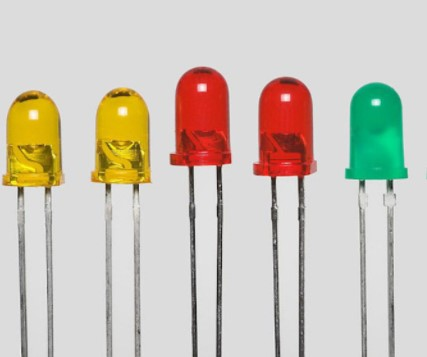
\includegraphics[width=0.3\textwidth]{h.jpg}
    \caption{LED bulbs}
    \label{fig:h}
\end{figure}

There are some several advantages that we can get from using LED bulbs.

\begin{itemize}
\item  Comparable in efficacy to CFLs, gaining on fluorescent tubes, and incandescents.
\item  Fixtures are directional, allowing for more efficient
optics.
\item  Quality of White Light LEDs now comparable to CFLs,
recent advances assure better consistency in color and CCT.
\item  Significantly longer Useful life.
\item  No infrared, (IR) radiation.
\item  Can operate in cold environments.

\end{itemize}

additionally, metal contacts and container were used during the experiment. 

\chapter{METHODOLOGY}
\section{Circuit Diagram}

This section demonstrates basic water level indicator circuits with LED lights. The given circuits was shown  here  are simple and built using transistors, LEDs and  resistors. 

\begin{figure}[hbt!]
    \centering
    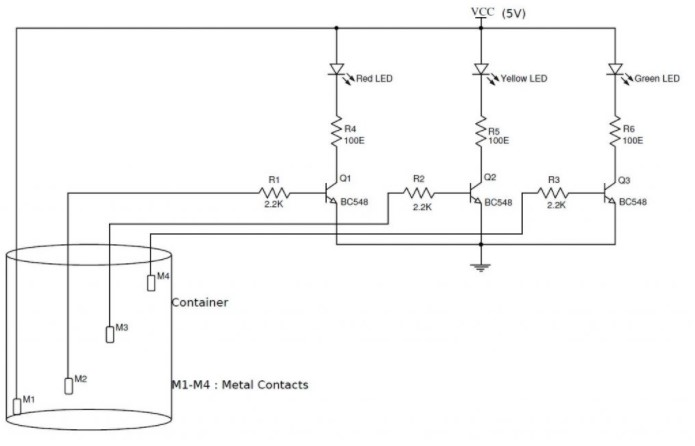
\includegraphics[width=1.0\textwidth]{i.jpg}
    \caption{Circuit diagram}
    \label{fig:i}
\end{figure}

\newpage
\section{Project Methodology}
The circuit is designed to signify four levels of water contained in the tank. Low but not empty, half and full but not overflowing. Since there is no water in the tank, all the LEDs are off to show that the tank is absolutely empty. When the water level rises and the sensor is touched, the Red LED will blink indicating that there is water inside the tank. When the water level begins to increase and hits 
half of the tank, the Yellow LED, Green LED may glow. Whenever the water in the tank rises to full a warning is made by the buzzer to show that the tank is full and  the White LED may glow.

\section{Project Procedures}
First BC547 transistor was inserted on the breadboard. The left one is collector, the middle one is base and the last one is the emitter. Then the other two transistors were inserted as well on the breadboard. After that 100$\Omega$ and 1k$\Omega$ resistors were connected to all the base and collector terminals of the transistor of the breadboard in respectively. Next the Red LED with its anode to the emitter of first transistor was inserted and cathode to the negative rail of the breadboard and do the same step for Green, Yellow and White LEDs as well. Then the buzzer was connected on the breadboard and  the negative wire of the buzzer was connected to the negative rail of the breadboard and positive wire to the emitter of the third transistor. After that one wire was connected each to the base of the transistors. And also the other end was dipped of the wire in the container with water, it is important to dip the wires in the water level-wise and not keep the bare ends of the wire on the same level. Finally the power was connected to the circuit and start adding water to the container and see the LED's light up sequentially and the buzzer buzzing at the end. 



\subsection{Circuit Working}
Here we are using transistor(npn) as a switch. Initially there is no voltage applied to the base of the transistor $T_{1}$ and the transistor is in OFF state. And also no current is flowing through collector emitter and LED is OFF. When the water level reaches to point A in the tank, the positive side of the battery gets connected to the bases of the transistor $T_1$ through the water. Hence when a positive voltage applied to the base of the transistor $T_1$, it gets into ON state and current starts flowing from the collector to emitter. Then Red LED blinks. Here why we used resistors at the base of each transistor, to limit the maximum base current. Basically a transistor gets its ON state fully when a voltage of 0.7V is applied to the base. There are resistors with each of the LEDs to drop the voltage across LEDs, otherwise LED may blow up. Also same phenomenon happens when water level reaches to point B and point C. As soon as water level reaches to point B and point C a positive voltage gets applied to the transistor $T_2$ and $T_3$ in respectively. Finally what we can see, buzzer beeps when water level reaches to D.  


\subsection{Calculation}

\begin{figure}[hbt!]
    \centering
    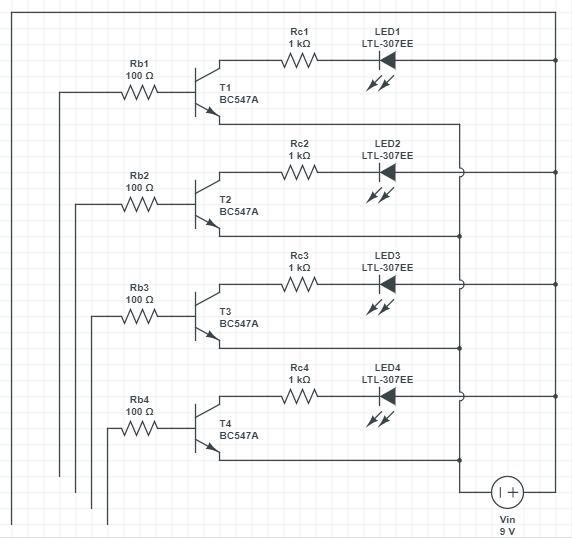
\includegraphics[width=0.8\textwidth]{l.jpeg}
    \caption{Diagram of circuit}
    \label{fig:my_label}
\end{figure}

\newpage
\begin{table}[h]
\centering
\begin{tabular}{|p{4cm}|p{4cm}|}
\hline
$\textbf{Component}$ & $\textbf{Value}$ \\ \hline
		$R_{B_{1-4}}$ & 100$\Omega$\\ \hline
 		$R_{C_{1-4}}$ & 1k$\Omega$\\ \hline
		$LED_{1-4}$   & LTL-307EE\\ \hline
		$T_{1-4}$     & BC547\\ \hline
		
\end{tabular}
\caption{Values of components}
\label{tab:1}
\end{table}

Resistance of drinking water is (2-200)$\Omega$m

\textbf{LTL-307EE} forward voltage is 2V

When \textbf{BC547} transistor \underline{BE} in on, 

\begin{center}
\begin{equation*}
V_{CE}=5V 
\end{equation*}
\begin{equation*}
I_{C}=2mA
\end{equation*}
\end{center}

\begin{figure}[hbt1]
    \centering
    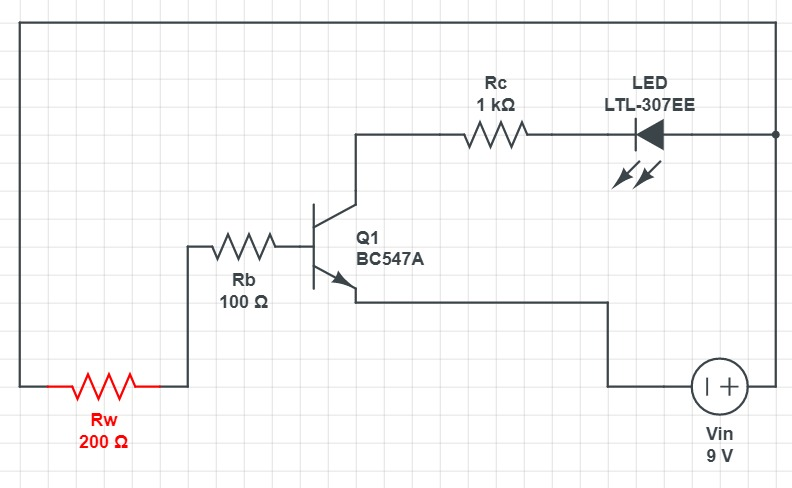
\includegraphics[width=0.9\textwidth]{k.jpeg}
    \caption{Consider ABCE loop}
    \label{fig:k}
\end{figure}

\newpage

Calculating the current flowing through the collector (\textbf{$I_{C}$}) 

Applying KVL for ABCE Loop ,
\begin{center}
	\begin{equation}
	V_{L1}+I_{C}R_{C}+V_{CE} = V_{i}
	\end{equation}
	\begin{equation*}
	2V+1\times10^{-3}I_{C}V+5V = 9V
	\end{equation*}
	\begin{equation*}
	I_{C}=2\times10^{-3}A
	\end{equation*}
	\begin{equation*}
	I_{C}=2mA
	\end{equation*}
\end{center}
Let assume {$V_{BE_{max}}$} = 0.7V
\\
Calculating the current flowing through the Base (\textbf{$I_{B}$}) 

Applying KVL for FBEA Loop,

\begin{center}
\begin{equation}
I_{B}R_{W}+I_{B}R_{B}+V_{BE}=V_{i}
\end{equation}
\begin{equation*}
200I_{B}V+100I_{B}V+0.7V=9V
\end{equation*}
\begin{equation*}
300I_{B}V=8.3V
\end{equation*}
\begin{equation*}
I_{B}=27.7mA
\end{equation*}
\end{center}

\newpage

\subsection{Application}
There are many of application of water level indicator where we can see in our day today life. Some are, The water level indicator is used in hotels, home apartments. complex and in factories as well. Automatically the pump will switch ON/OFF when the water level in the tank is empty and full. Also we can measure the fuel level in motor vehicles. The liquid level containers huge in the companies. 

\subsection{Advantages}'
By using water level indicator we will able to get many of advantages and few of disadvantages. The water level indicators are low cost in the market, any person can identify the water level easily by hearing the beep sound, and by using this we will able to control the water level safely and easily. These are the things we can defined as advantages through this. When consider the LED bulbs those are easily damage when currents flow and t is sensitive to environment like humidity temperature. Then we have to replace LED bulbs time to time. 

\newpage

\chapter{DISCUSSION}
In fact, the level of any conductive non-corrosive liquids can be measured using this circuit.  Use good quality insulated Aluminum wire for probes. Here, We can use any simple npn transistor. In this case we have used BC547 transistors. We have used 9V DC battery in the circuit simulation. But, In practical usage, It's better to use AC current, because electrolysis could happen at the probes. In addition to that, We may have to adjust the resistor values because of the conductivity of water could be vary due to conditions of the water source. In future upgrade we could use conductor relay switch, because it doesn't take much current to function then we can completely avoid the water conductivity problem.



\newpage

\chapter{CONCLUSION}
The water level indicator is the best electronic water level starter and saves water accordingly. The led blinks according to their amount of water reaches them and shows the buzzing sound to avoid pouring when it reaches its final threshold.



\end{document}
